\section{Zigbee} % Zigbee
\subsection{Descripción} % Descripcion
Zigbee es un protocolo desarrollado por la organización Zigbee Alliance, que ofrece una solución para comunicaciones inalámbricas bidireccionales, de bajo coste y bajo consumo de energía. Las soluciones que aporta Zigbee se pueden emplear en diferentes campos: controles industriales, automatización de viviendas y edificios, aplicaciones de sensores médicos, etc. Zigbee está basado en el estándar IEEE 802.15.4, apoyándose en las capas PHY y MAC definidas por el estándar.
\\\\Zigbee define la comunicación a partir del nivel 3 de la capa OSI, proporcionando la capa de red (NWK) y el framework (AF) para la capa de aplicación (APL). Este framework consiste en la subcapa de soporte de aplicación (APS), que define perfiles Zigbee, clusters y endpoints, y la subcapa de objetos de dispositivos Zigbee (ZDO), que proporciona funcionalidades de descubrimiento de dispositivos y gestión de seguridad y redes. Los objetos de aplicación definidos por los fabricantes utilizan el framework y comparten los servicios de seguridad y soporte de aplicación con el ZDO.
\\\\ En la siguiente figura se muestra un esquema general de la pila del protocolo Zigbee:
\begin{figure}[H]
\centerline{\includegraphics[width=15cm]{figuras/zigbeestack.eps}}
\caption{Pila del protocolo Zigbee \cite{especificacionzigbee}}
\label{pilazigbee}
\end{figure}
\clearpage




\subsection{Características} % Caracteristicas
El protocolo Zigbee tiene una serie de características que lo diferencian del resto de soluciones para redes inalámbricas de área personal. Estas características hacen que sea uno de los protocolos más utilizados en entornos industriales de IoT:
\begin{itemize}
\item Las redes Zigbee pueden componerse de una gran cantidad de dispositivos, como máximo 65535 nodos distribuidos en subredes de 255.
\item Los dispositivos que implementan Zigbee requieren un menor consumo de energía que los dispositivos que implementan otros protocolos, debido a que estos pueden permanecer dormidos la mayor parte del tiempo. En términos exactos, Zigbee tiene un consumo de 30 mA cuando el dispositivo está transmitiendo información y 3$\mu$A en reposo, lo que alarga la vida útil de las baterías.
\item Permite una velocidad de transmisión de datos de hasta 250 kbit/s en la banda de frecuencia de 2.4 GHz.
\item El rango de transmisión es bastante elevado, oscilando entre 10 y 75 metros dependiendo del entorno.
\item La batería de los dispositivos dura meses o incluso años sin tener que ser reemplazada.
\item Los paquetes que se transmiten por la red son muy pequeños, comparados con otros protocolos utilizados en IoT como Wifi o Bluetooth.
\end{itemize}
\clearpage




\subsection{Tipos de dispositivos} % Tipos de dispositivos
Una red Zigbee puede estar formada por diferentes dispositivos/nodos:
\\\\$\blacksquare$ {\underline{\textbf{Coordinador}}}
\\\\El coordinador es el componente principal de la red Zigbee, el cual gestiona la red y proporciona los controles de seguridad en la misma. Este componente actúa normalmente como un {\it centro de confianza} (TC, Trust Center). El coordinador es un elemento imprescindible para formar una red Zigbee y debe estar conectado a la corriente, ya que no puede estar inactivo.
\\\\$\blacksquare$ {\underline{\textbf{Enrutador}}}
\\\\El enrutador actúa como un nodo intermedio entre el coordinador y los dispositivos finales. Su función es redirigir el tráfico entre varios dispositivos, retransmitiendo los datos que recibe. Los enrutadores no pueden dormir (estar inactivos), al igual que el coordinador. Estos dispositivos primero se unen a la red con el permiso del coordinador y posteriormente son capaces de permitir a otros enrutadores y dispositivos finales unirse a la red.
\\\\$\blacksquare$ {\underline{\textbf{Dispositivo final}}}
\\\\Los dispositivos finales son componentes simples de baja potencia que están alimentados por baterías. Estos dispositivos no poseen las funcionalidades de los enrutadores ni del coordinador, sólo se pueden comunicar con otros dispositivos a través de sus nodos padre. A diferencia del coordinador y los enrutadores, los dispositivos finales no consumen practicamente energía debido a que pueden permanecer dormidos y despertarse en segundos cuando se requiere su uso. Ejemplos de estos dispositivos son los sensores de movimiento, las bombillas inteligentes, etc. 
\\\\$\blacksquare$ {\underline{\textbf{Centro de confianza Zigbee (ZTC, Zigbee Trust Center)}}}
\\\\El ZTC es un dispositivo que proporciona la gestión de la seguridad en una red Zigbee. Este dispositivo elige el canal a usar por los dispositivos en las comunicaciones, permite el acceso de otros dispositivos a la red, realiza un seguimiento de los dispositivos y habilita la seguridad de extremo a extremo entre ellos. Aunque la funcionalidad más importante es que almacena y distribuye las claves de red, imprescindibles para la seguridad de la misma.
\\\\$\blacksquare$ {\underline{\textbf{Puerta de enlace Zigbee (Zigbee gateway)}}}
\\\\Es usada para conectar la red Zigbee con otras redes, como una LAN, mediante la conversión del protocolo.
\clearpage




\subsection{Topologías de la red} % Topologías de la red
El protocolo Zigbee permite tres tipos de formaciones de una red:\vspace{0.4cm}
\begin{itemize}
\item{\bf Topología en estrella:} la red es controlada por un sólo dispositivo, el coordinador Zigbee, responsable de iniciar y mantener el resto de nodos de la red. En esta topología, los dispositivos finales solo se comunican con el coordinador, lo que puede provocar un cuello de botella, ya que todos los paquetes de datos deben de pasar por el coordinador. La ventaja de utilizar esta topología es que los paquetes realizan como mucho dos saltos para llegar a su destino.\vspace{0.4cm}
\item{\bf Topología en árbol:} el coordinador ZigBee es responsable del inicio de la red y de la elección de ciertos parámetros clave de la red. La red puede ampliarse mediante el uso de enrutadores ZigBee, los cuales mueven los datos y controlan los mensajes a través de la red, utilizando una estrategia de enrutamiento jerárquico donde el coordinador y los enrutadores son los nodos padre de la red y los dispositivos finales son los nodos hijo.\vspace{0.4cm}
\item{\bf Topología de malla:} el coordinador ZigBee es responsable del inicio de la red y de la elección de ciertos parámetros clave de la red. La red puede ampliarse mediante el uso de enrutadores ZigBee. Es el equivalente a la topología punto a punto en IEEE 802.15.4 (Fig. \ref{ieeetopologiamalla}). En este tipo de redes, los dispositivos que participan en la retransmisión de los mensajes son solo FFDs. Los RFDs pueden formar parte de la red pero únicamente se pueden comunicar con un dispositivo en particular (coordinador o enrutador).
\vspace{0.5cm}
\end{itemize}
\begin{figure}[H]
\centerline{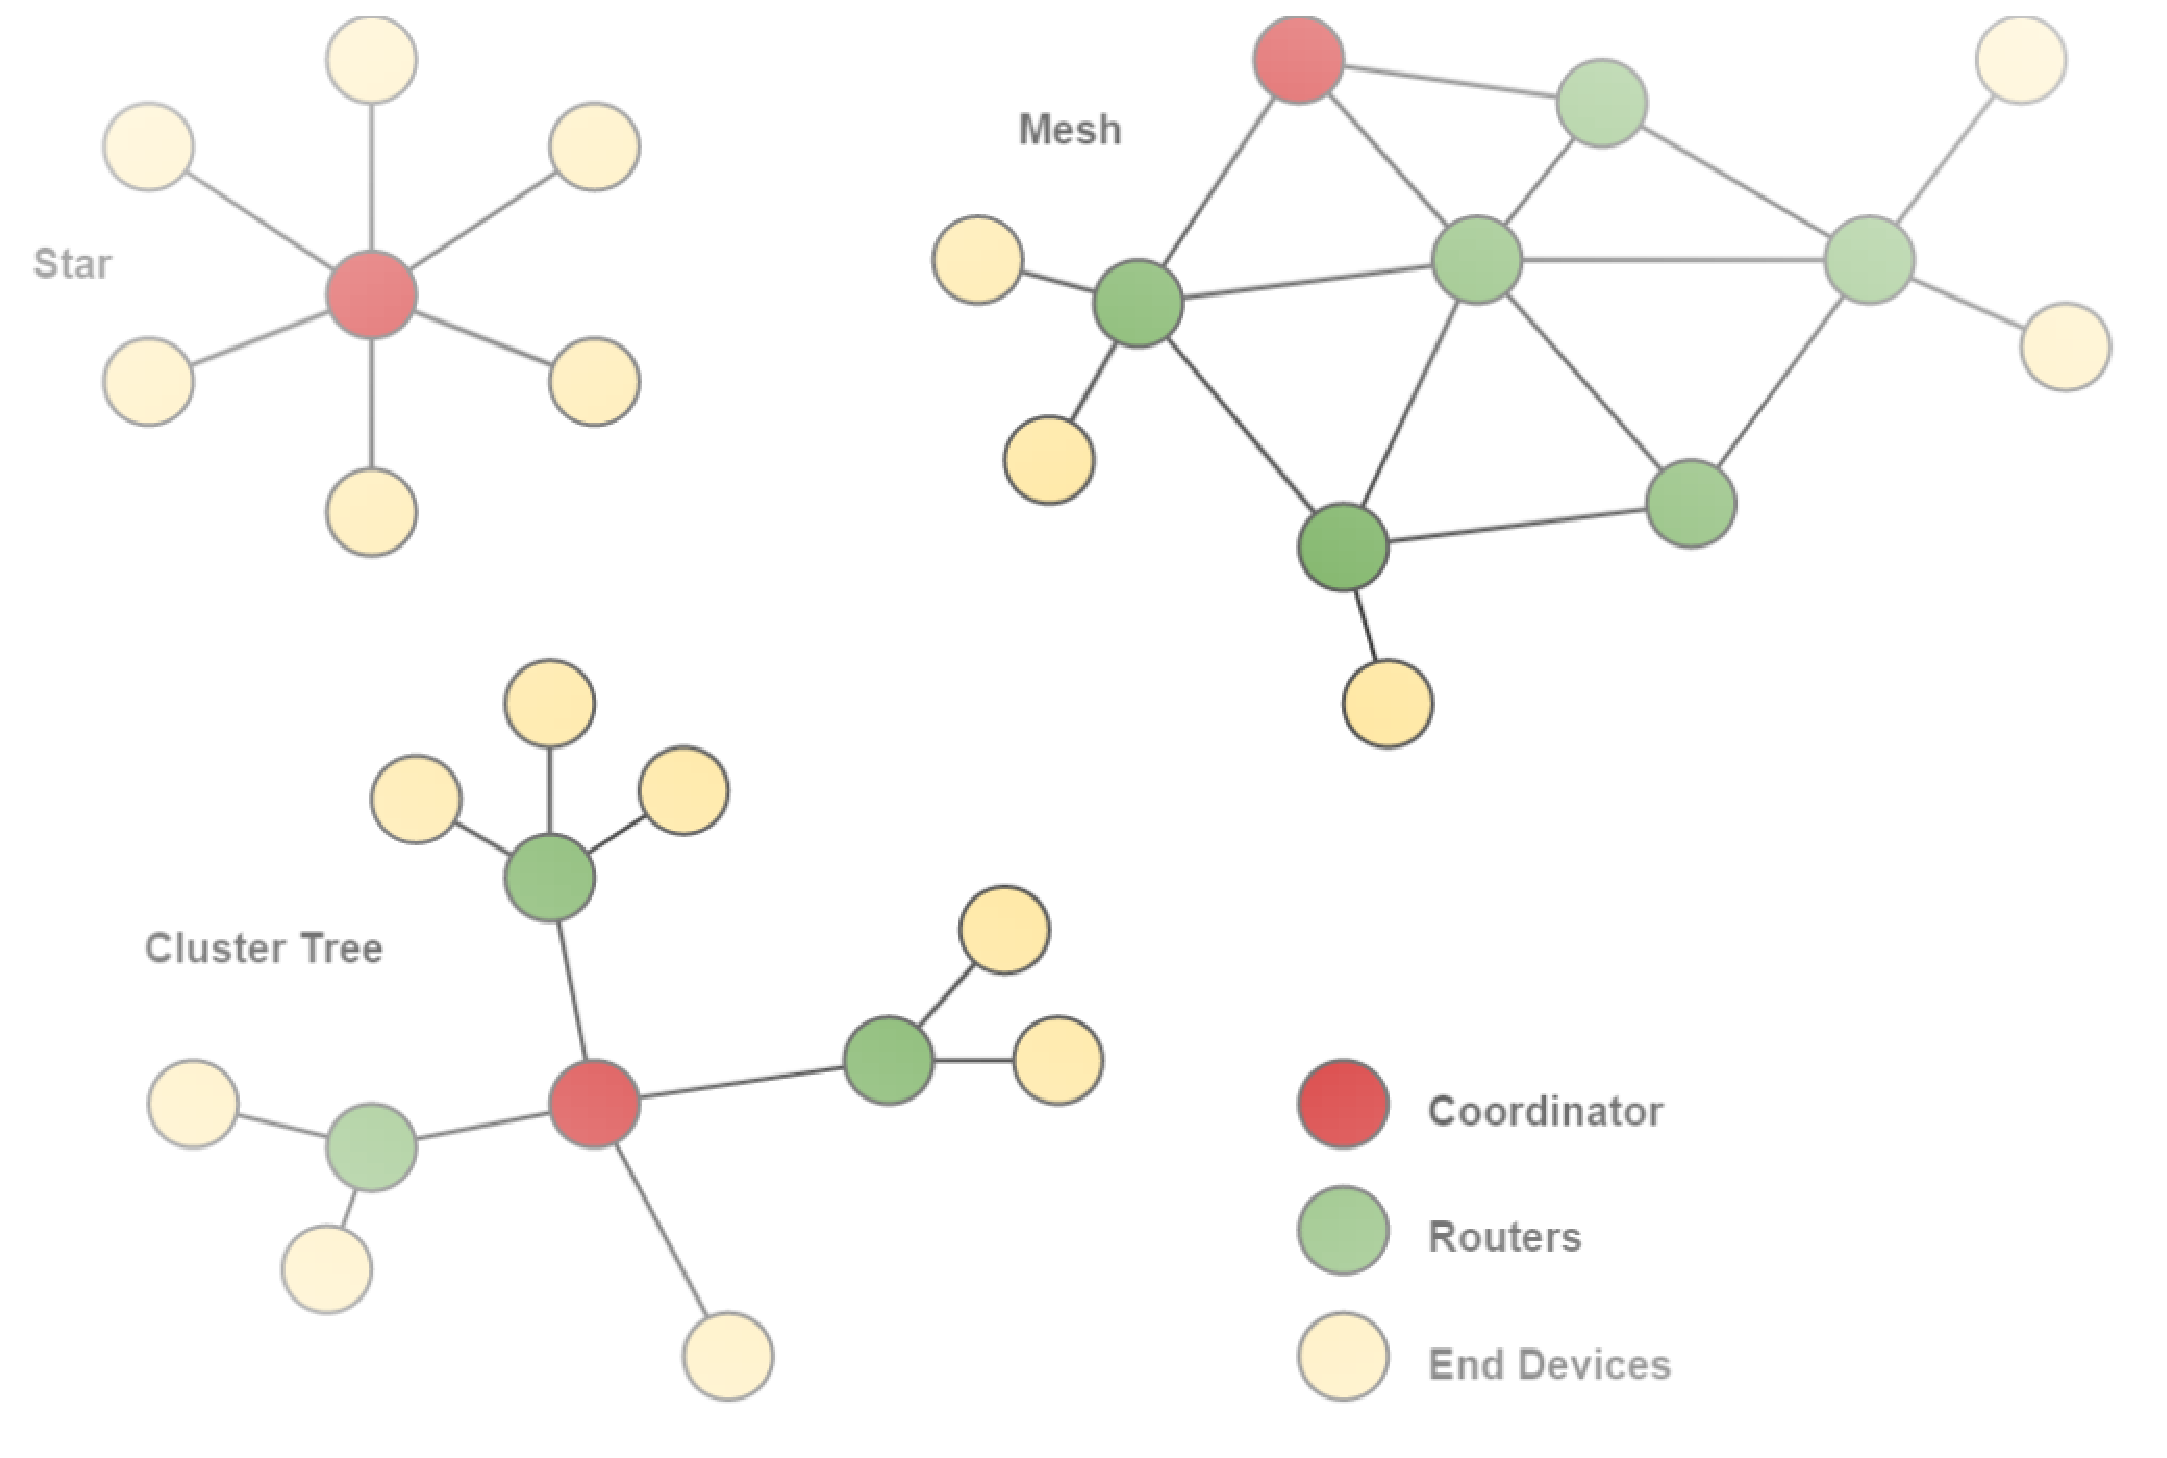
\includegraphics[width=12cm]{figuras/topologiaszigbee.eps}}
\caption{Topologías de la red Zigbee \cite{zigbeetopologias}}
\label{topologiaszigbee}
\end{figure}
\clearpage




\subsection{Arquitectura} % Arquitectura
Zigbee construye a partir del estándar IEEE 802.15.4 la totalidad de la pila del protocolo, añadiendo una serie de capas y funcionalidades.
\subsubsection{{\large Capa de red (NWK)}} % Capa de red (NWK)
Para interactuar con la capa de aplicación, la capa de red incluye conceptualmente dos entidades de servicio que proporcionan las operaciones necesarias para la comunicación entre capas:
\begin{itemize}
\item{\bf Entidad de servicio de datos (NLDE):}  proporciona el servicio de transmisión de datos, permitiendo transportar unidades de datos entre dos o más dispositivos ubicados en la misma red. La NLDE ofrece los siguientes servicios:
	\begin{itemize}
	\item{\bf Generación de la unidad de datos del protocolo de nivel de red (NPDU):} a partir de la unidad de datos del protocolo generada por la subcapa de soporte de aplicación, la NLDE es capaz de generar el NPDU.
	\item{\bf Enrutamiento específico de la topología:} es capaz de transmitir un NPDU a un dispositivo que sea el destino final de la comunicación o sea el siguiente paso hasta el destino final en la cadena de comunicación.
	\item{\bf Seguridad:} tiene la capacidad de asegurar la autenticidad y la confidencialidad en una transmisión de datos.
	\end{itemize}
\item{\bf Entidad de servicio de gestión (NLME):} permite a una aplicación interactuar con la pila del protocolo. La NLME ofrece los siguientes servicios:
	\begin{itemize}
	\item{\bf Configuración de un nuevo dispositivo:} se realizan las configuraciones necesarias para que un dispositivo se una a la red Zigbee existente.
	\item{\bf Crear una red:} capacidad para establecer y formar una red desde cero.
	\item{\bf Unirse, re-unirse, y abandonar una red:} proporciona a un dispositivo la capacidad para unirse, volver a unirse, o abandonar una red. También ofrece la posibilidad a coordinadores y enrutadores de enviar un mensaje a un dispositivo para que abandone la red.
	\item{\bf Direccionamiento:} se asignan dos identificadores a los dispositivos de la red: una dirección única de 64 bits a nivel de enlace (MAC) asignada por el fabricante, y una dirección de 16 bits (dirección lógica o de red).
	\item{\bf Descubrimiento de vecinos:} capacidad para descubrir, guardar y notificar información de los ''vecinos'' de un dispositivo.
	\item{\bf Descubrimiento de ruta:} proporciona la capacidad de descubrir y registrar caminos a través de la red, realizando un enrutamiento.
	\item{\bf Control en recepción:} permite a un dispositivo controlar cuando se activa el receptor y por cuánto tiempo, sincronizándose la capa MAC.
	\end{itemize}
\end{itemize}
\vspace{0.8cm}
Cuando un nodo enrutador o dispositivo final quiere unirse a la red Zigbee, le envía un mensaje al coordinador preguntándole por una dirección de red para realizar el proceso de asociación y realizar el enrutado de la información de la red utilizando esa dirección. Posteriormente, este puede enviar información a sus nodos hermanos a través de los enrutadores que se encuentran siempre despiertos esperando paquetes.



\subsubsection{{\large Capa de aplicación (APL)}} % Capa de aplicación
La capa de aplicación está formada por tres componentes principales, los cuales proporcionan las funcionalidades necesarias para el correcto manejo de las aplicaciones:
\begin{itemize}
\item{\bf Subcapa de soporte de aplicación (APS)}: proporciona una interfaz entre la capa de red y la capa de aplicación, a través de un conjunto de servicios generales que son utilizados por el ZDO y los objetos de aplicación. Los servicios de esta subcapa son proporcionados por dos entidades:
	\begin{itemize}
	\item{\bf Entidad de datos de la subcapa APS (APSDE):} proporciona un servicio de datos a la capa de red y a los objetos de aplicación, permitiendo el transporte de las PDUs entre dos o más dispositivos. También se encarga de la fragmentación y el rechazo de mensajes duplicados.
	\item{\bf Entidad de gestión de la subcapa APS (APSME):} proporciona un servicio de gestión para permitir a una aplicación interactuar con la pila del protocolo, realizando la gestión de la asociación, la gestión de grupos y la gestión de las relaciones entre dispositivos.
	\end{itemize}
\item{\bf Framework de aplicación (AF):} es el entorno en el que están alojados los objetos de aplicación de dispositivos Zigbee. Se pueden definir hasta 254 objetos de aplicación distintos, disponiendo cada uno de ellos de un punto de acceso (endpoint). El endpoint 0 se reserva para la interfaz de datos con el ZDO, y el 255 para la función de envío mensajes de broadcast a todas las aplicaciones de un dispositivo.
El AF utiliza los siguientes conceptos para llevar a cabo la gestión de las aplicaciones:
	\begin{itemize}
	\item{\bf Perfiles de aplicación:} son acuerdos para determinar el formato de los mensajes y las acciones de procesamiento. Estos perfiles de aplicación permiten a las aplicaciones enviar comandos, pedir datos y procesar comandos y respuestas.
	\item{\bf Clústeres:} son reconocidos por un identificador de clúster, el cual está asociado con un flujo de datos desde o hacia un dispositivo.
	\end{itemize}
\item{\bf Los objetos de dispositivos Zigbee (ZDO)}: representan una clase base de funcionalidades que proporcionan una interfaz entre los objetos de aplicación, los perfiles de dispositivos y la APS. Existe un perfil definido para el ZDO denominado perfil de dispositivo Zigbee o ZDP, el cual contiene los descriptores del dispositivo y los clústeres con los que puede operar.
\end{itemize}
\clearpage




\subsection{Seguridad en redes Zigbee} % Seguridad en redes Zigbee
En este punto se explican las medidas de seguridad implementadas por el protocolo Zigbee en las capas de red y aplicación, complementando los servicios de seguridad de IEEE 802.15.4. ZigBee se considera un protocolo de comunicación seguro debido a los servicios de seguridad que proporciona: establecimiento seguro de claves, transporte seguro de claves, protección de tramas mediante criptografía simétrica y gestión segura de dispositivos.
\subsubsection{Supuestos de Seguridad} % Supuestos de seguridad
La seguridad de Zigbee se basa en las siguientes suposiciones inherentes:
\begin{itemize}
\item{\bf Confianza abierta:} se asume un modelo de confianza en el que las capas de la pila del protocolo confian entre sí. Por lo tanto, la protección criptográfica solo existe entre dispositivos, pero no entre capas. La capa que origina una trama es responsable de asegurarla inicialmente.
\item{\bf Almacenamiento de claves simétricas:} Zigbee asume que las claves secretas que se utilizan, no se encuentran disponibles fuera del dispositivo de forma no segura. Un dispositivo no transmititá las claves a otro dispositivo a menos que se envíen de forma cifrada, como durante el transporte de clave (key-transport). Sin embargo, durante el transporte inicial, la clave utilizada para la protección puede ser conocida, produciéndose un breve momento de vulnerabilidad donde cualquier dispositivo podría escuchar el medio de transmisión y obtener dicha clave. Además, el acceso físico al dispositivo puede permitir la obtención de las claves utilizadas en la red u otra información sensible.
\item{\bf Protección empleada:} todos los nodos routers y dispositivos finales deben adaptarse al esquema de seguridad empleado por la red, en un modelo de seguridad distribuida o centralizada.
\item{\bf Mecanismos criptográficos y políticas de seguridad:} se supone que los desarrolladores de Zigbee siguen los estándares de protección de las comunicaciones y aplican estos mecanismos de forma correcta.
\item{\bf Hardware seguro:} se asume que el hardware de los dispositivos es resistente a la manipulación y al acceso físico.
\end{itemize}
Teniendo en cuenta las suposiciones sobre la seguridad del protocolo, se deben explorar y tener muy en cuenta los modelos de seguridad, las claves utilizadas para la comunicación, la gestión de las claves, y otros mecanismos de seguridad como autenticación, protección de ataques de repetición, etc.
\clearpage




\subsubsection{Modelos de Seguridad} % Modelos de Seguridad
Zigbee proporciona la implementación de dos modelos de seguridad de red. Estos se diferencian en la manera de admitir nuevos dispositivos y en cómo protegen la información transmitida:
\begin{itemize}
\item{\bf Modelo de seguridad centralizado:} es complejo pero proporciona mayor seguridad. En este modelo hay un Centro de Confianza (TC) que se encarga de formar la red, además de configurar y autenticar a los routers y dispositivos finales. El TC establece una Clave de Enlace de Centro de Confianza (TCLK) única para cada dispositivo de la red a medida que se unen, y vincula las claves para cada par de dispositivos. Además, todos los nodos deben preconfigurarse con una clave de enlace, cifrando la clave de red al ser enviada desde el TC a los dispositivos que desean unirse.
\item{\bf Modelo de seguridad distribuido:} es un modelo más simple y menos seguro ya que no hay un TC singular en la red. Los routers, los cuales pueden actuar como TCs distribuyendo las claves de red, y los dispositivos finales son los encargados de formar la red. Para participar en redes de seguridad distribuida, los dispositivos deben estar preconfigurados con una clave de enlace utilizada para cifrar la clave de red, cifrando los mensajes entre nodos con esta última.
\end{itemize}
\begin{figure}[H]
\centerline{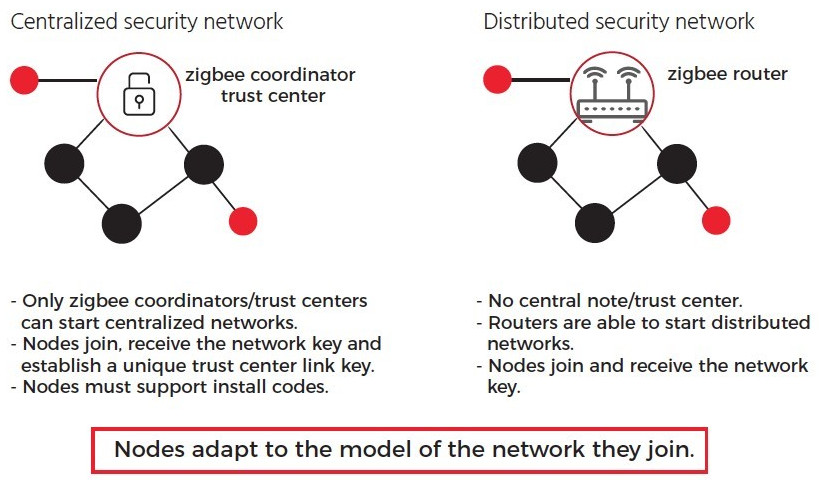
\includegraphics[width=8cm]{figuras/zigbeemodels.jpeg}}
\caption{Modelos de Seguridad centralizado y distribuido \cite{analisisseguridadzigbee}}
\label{modeloscentraldistribuida}
\end{figure}
\subsubsection{Políticas de Seguridad} % Políticas de seguridad
Un TC puede actuar de dos modos al seguir los dos tipos de políticas de seguridad que define Zigbee:
\begin{itemize}
\item{\bf Modo Comercial:} el TC almacena los tres tipos de claves y las comparte con cualquier dispositivo de la red. Este modo requiere recursos de memoria elevados ya que se almacena una lista de dispositivos y claves, pero ofrece un modelo centralizado completo para el control de la seguridad de las claves.
\item{\bf Modo Residencial:} el TC comparte únicamente la clave de red y el resto de información se almacena en los nodos. Este es el modo más usado en las redes de sensores inalámbricas, debido a que los dispositivos normalmente poseen recursos de memoria bajos.
\end{itemize}
\clearpage




\subsubsection{Claves de Seguridad} % Claves de seguridad
ZigBee fundamenta su seguridad en la utilización de criptografía de clave simétrica, contando con un elaborado protocolo para la gestión de dichas claves. Se utilizan 3 tipos distintos de claves simétricas (cada una de 128 bits de longitud) según se asocien a una red, a un grupo de dispositivos o bien a un enlace entre dos elementos:
\begin{itemize}
\item{\bf Claves Maestras (Master Keys):} son claves, únicamente utilizadas por la APS, de las cuales derivan las diferentes claves de enlace. Debido a su importancia, este tipo de claves solo se obtienen mediante métodos seguros: preinstalación (por ejemplo, durante la instalación de fábrica) o transporte de claves (el dispositivo hace una petición al TC para que le envíe la clave).
\item{\bf Claves de Enlace (Link Keys):} son claves únicas entre cada par de nodos, gestionadas por el nivel de aplicación. Se utilizan para cifrar las comunicaciones punto a punto entre cada par de dispositivos a nivel de aplicación y para minimizar los riesgos de seguridad relacionados con la transmisión de la clave maestra. Zigbee define varios tipos de claves de enlace:
	\begin{itemize}
	\item{\bf Clave de enlace global}: utilizada por el centro de confianza y los nodos.
	\item{\bf Clave de enlace única}: determina cómo maneja el dispositivo los mensajes del centro de confianza (comandos APS).
	\end{itemize}
\item{\bf Claves de Red (NWK Keys):} son claves únicas, compartidas entre todos los nodos de la red. Se generan por el TC y se cambian cuando finaliza un determinado intervalo de tiempo. Cuando el TC decide modificar la clave de red, la nueva clave se difunde de manera cifrada con la clave antigua, restableciendo los contadores de trama de los dispositivos. Los nodos necesitan obtener esta clave para unirse a la red y comunicarse de forma segura con otros dispositivos. Zigbee define dos tipos de transmisión de la clave de red: estándar (la clave viaja en texto plano) y alta seguridad (la clave se encripta antes de enviarse).
\end{itemize}
\subsubsection{Seguridad en redes distribuidas y centralizadas} % Seguridad en redes distribuidas y centralizadas
Según el modelo de seguridad implementada, se utilizan diferentes tipos de claves para administrar la seguridad de la red Zigbee. En un modelo de seguridad distribuido se utilizan las siguientes claves:
\begin{itemize}
\item{\bf Clave de red}: descrita anteriormente.
\item{\bf Clave de enlace global para el modelo seguridad distribuida}: se utiliza para cifrar las comunicaciones entre el router padre y el nodo que quiera unirse a la red de seguridad distribuida.
\item{\bf Clave de enlace única preconfigurada}: se utiliza también para cifrar las comunicaciones entre el router padre y el nodo que quiera unirse a la red.
\end{itemize}
Las claves utilizadas en el modelo se seguridad centralizada se definen a modo de resumen en la siguiente tabla:
\clearpage
\begin{table}[h!]
\begin{tabular}{|l|l|l|}
\hline
\rowcolor[HTML]{A1C9F0} 
\multicolumn{1}{|c|}{\cellcolor[HTML]{A1C9F0}\textbf{Claves de seguridad}}                  & \multicolumn{2}{c|}{\cellcolor[HTML]{A1C9F0}\textbf{Descripción}}                                                                                                                                                                                                                                                                                                                                                                                                                                                                                                       \\ \hline
\multicolumn{3}{|l|}{\textbf{Seguridad nivel de red}}                                                                                                                                                                                                                                                                                                                                                                                                                                                                                                                                                                                                                 \\ \hline
\multicolumn{1}{|c|}{\textit{Clave de red}}                                                 & \multicolumn{2}{l|}{\begin{tabular}[c]{@{}l@{}}• Clave esencial para cifrar las comunicaciones entre todos los\\ nodos de la red.\\ • Generada aleatoriamente por el centro de confianza (TC).\\ • Distribuida a los nodos entrantes, cifrada con una clave de\\ enlace preconfigurada.\end{tabular}}                                                                                                                                                                                                                                                                       \\ \hline
\multicolumn{3}{|l|}{\textbf{Seguridad nivel de aplicación}}                                                                                                                                                                                                                                                                                                                                                                                                                                                                                                                                                                                                          \\ \hline
\textit{\begin{tabular}[c]{@{}l@{}}Clave de Enlace Global\\ (preconfigurada)\end{tabular}} & \multicolumn{2}{l|}{\begin{tabular}[c]{@{}l@{}}• Usada entre el centro de confianza y el resto de nodos.\\ • Preconfigurada en todos los nodos (excepto cuando \\ se preconfigura una clave de enlace única).\\ • Usada al unirse nuevos dispositivos para cifrar la clave de red\\ transportada desde el centro de confianza a los nodos.\\ • Si es definida por ZigBee, permite la adición a la red de nodos\\ de distintos fabricantes. {\small (0x5A 0x69 0x67 0x42 0x65 0x65 0x41 0x6C}\\{\small  0x6C 0x69 0x61 0x6E 0x63 0x65 0x30 0x39 (ZigbeeAlliance09))} \\ • Si es definida por el fabricante, permite la adición de nodos\\ pertenecientes a dicho fabricante.\end{tabular}}        \\ \hline
\multicolumn{1}{|c|}{\textit{Clave de Enlace Única}}                                        & \multicolumn{2}{l|}{\begin{tabular}[c]{@{}l@{}}Clave opcional utilizada para cifrar las comunicaciones entre un\\ par de nodos. Puede ser de los siguientes tipos:\end{tabular}}                                                                                                                                                                                                                                                                                                                                                                                        \\ \hline
                                                                                            & \textit{\begin{tabular}[c]{@{}l@{}}Clave de enlace única \\ preconfigurada\end{tabular}}          & \begin{tabular}[c]{@{}l@{}}• Usada entre el centro de\\ confianza y cualquier otro nodo.\\ • Preconfigurada en el centro de\\ confianza y el nodo.\\ • Se usa también para cifrar la\\ clave de red cuando se transporte\\ desde el centro de confianza al\\ nodo cuando intenta unirse.\end{tabular}                                                                                                                                                              \\ \hline
                                                                                            & \textit{\begin{tabular}[c]{@{}l@{}}Clave de Enlace del Centro\\ de Confianza (TCLK)\end{tabular}} & \begin{tabular}[c]{@{}l@{}}• Utilizada entre el centro de\\ de confianza y cualquier otro nodo.\\ • Se genera aleatoriamente por\\ el centro de confianza.\\ • Distribuida al nodo cifrada con\\ la clave de red y la clave de enlace\\ preconfigurada (si existe).\\ • Reemplaza a la clave de enlace\\ preconfigurada (si existe) pero la\\ aplicación debe guardar la clave\\ preconfigurada en caso de que\\ necesite volver a unirse a la red.\end{tabular} \\ \hline
                                                                                            & \textit{\begin{tabular}[c]{@{}l@{}}Clave de Enlace de\\ Aplicación\end{tabular}}                  & \begin{tabular}[c]{@{}l@{}}• Usada entre un par de nodos,\\ sin incluir al centro de confianza.\\ • Generada aleatoriamente por el\\ centro de confianza.\\ • Distribuida a cada uno de los\\ nodos cifrada con la clave de red y\\ la clave de enlace preconfigurada\\ (si existe).\end{tabular}                                                                                                                                                                  \\ \hline
\end{tabular}
\caption{Resumen Claves de Seguridad del modelo Centralizado \cite{analisisseguridadzigbee}}
\label{clavesmodelocentralizado}
\end{table}
\clearpage




\subsubsection{Arquitectura de Seguridad} % Arquitectura de Seguridad
La arquitectura del protocolo Zigbee también incluye mecanismos de seguridad en las capas de red y aplicación.
\\\\$\blacksquare$ \underline{\textbf{ Seguridad en la capa de red}}
\\\\La capa de red es responsable de los pasos necesarios para procesar las tramas entrantes y transmitir las tramas salientes de forma segura. Si se habilita la seguridad en esta capa, el mecanismo de protección de tramas utilizará el estándar de cifrado avanzado AES y CCM, siendo las capas superiores las encargadas de administrar la seguridad de esta capa configurando claves de red activas y determinando qué nivel de seguridad usar, además de establecer el contador de paquetes para prevenir ataques de repetición.
\\\\La capa de red utiliza claves de enlace si están disponibles o de lo contrario la clave de red activa para proteger los paquetes, añadiendo integridad a todo lo que haya por encima de la trama de red. 
\begin{figure}[H]
\centerline{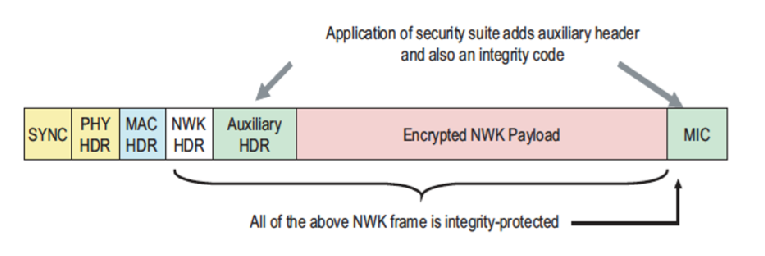
\includegraphics[width=10cm]{figuras/zigbeesecuritynwk.eps}}
\caption{Trama Zigbee con seguridad en la capa de red \cite{analisisseguridadzigbee}}
\label{tramazigbeenwk}
\end{figure}
$\blacksquare$ \underline{\textbf{ Seguridad en la capa de aplicación}}
\\\\Toda la seguridad de la capa de aplicación es gestionada por la subcapa APS. La APS permite que la seguridad de la trama se base en claves de enlace o en la clave de red, siendo responsable de proporcionar a las aplicaciones y al ZDO servicios de establecimiento de claves, transporte de claves y administración de dispositivos.
\begin{figure}[H]
\centerline{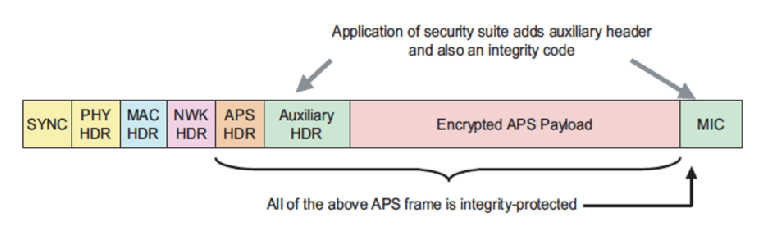
\includegraphics[width=10cm]{figuras/zigbeesecurityaps.eps}}
\caption{Trama Zigbee con seguridad en la capa de aplicación \cite{analisisseguridadzigbee}}
\label{tramazigbeeaps}
\end{figure}
\clearpage














